\chapter{Implementation and Iterative Usability Testing}
\label{chapter:Implementation}

The implementation phase of \ac{splash} involved translating the prototypes and data models into functional web applications. This phase was guided by a user-centered design approach, where iterative usability testing played a central role. As such, development was conducted in parallel with structured evaluation cycles, allowing continuous refinement of the interface and functionalities based on real-world user feedback.

\section{Application Architecture}

To address the distinct contexts and requirements of the primary user groups, two separate web applications were developed:

\begin{itemize}
    \item \textbf{SPLASH Lifeguard Application}: Designed for lifeguards and supervisors, this application supports core operational tasks such as:
    \begin{itemize}
        \item Team and shift scheduling;
        \item Hazard reporting and resolution;
        \item Real-time alerts and notifications;
        \item GPS-based tracking of beachgoers using smartbands;
        \item Access to beach history and performance metrics.
    \end{itemize}

    \item \textbf{SPLASH Beachgoer Application}: A public-facing interface optimized for mobile use, aimed at enhancing beach safety awareness and user autonomy. Key features include:
    \begin{itemize}
        \item Interactive map with live hazard zones;
        \item Reporting hazards directly from the beach;
        \item Access to flag status, weather updates, and UV index;
        \item Information on beach amenities and business locations;
        \item Integration with QR codes placed on-site.
    \end{itemize}
\end{itemize}

Both applications communicate with a centralized backend service and relational database (see Chapter~\ref{chapter:architecture}), ensuring data consistency, real-time synchronization, and secure access control across roles.

\begin{figure}[H]
    \centering
    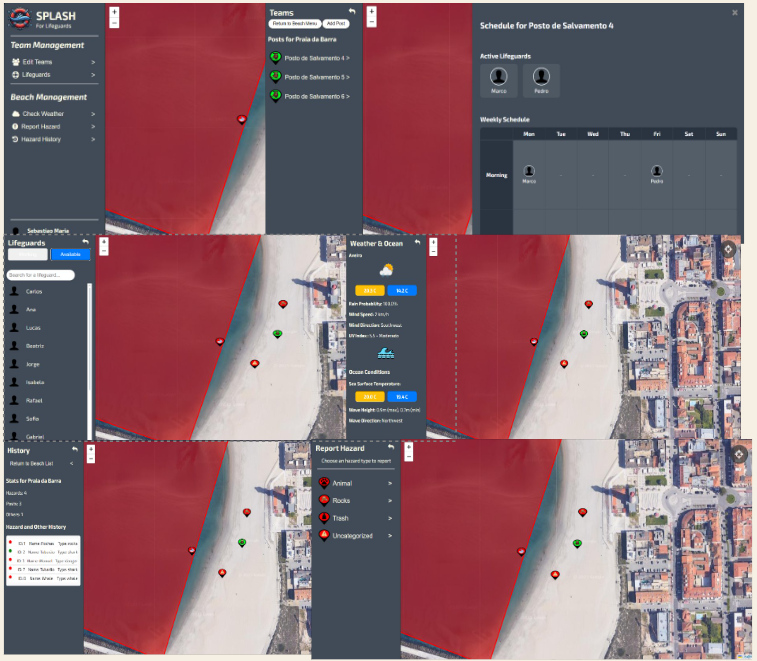
\includegraphics[width=15cm]{figs/pc.png}
    \caption{\textbf{\ac{splash} Web Interface} }
    \label{fig:splashwebinerface}
\end{figure}

\begin{figure}[H]
    \centering
    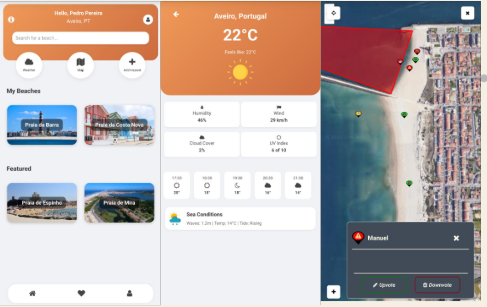
\includegraphics[width=15cm]{figs/mobile.png}
    \caption{\textbf{\ac{splash} Beachgoer Web Interface} }
    \label{fig:splashwebinerface}
\end{figure}


\section{Implementation Process}

The development followed an agile and incremental approach, allowing the integration of feedback loops after each testing phase. Initial mockups and user flows were implemented using ReactJS for the frontend and Node.js/Express for the backend services. Data was stored in a PostgreSQL database designed according to the relational schema presented earlier.

Security measures were implemented to protect personal and location data, complying with privacy and ethical guidelines, particularly regarding GPS tracking and emergency notifications.

\section{Iterative Usability Testing}

Following the initial Wizard of Oz evaluation (Chapter~\ref{chapter:Usability}), two subsequent rounds of usability testing were conducted with improved prototypes:

\subsection{Post-Implementation Test Plan}

\begin{itemize}
    \item \textbf{Participants:} Five individuals from the original pool were re-invited to test the functional prototypes, ensuring continuity in feedback. The profiles again covered all main personas.

    \item \textbf{Test Scenarios:} Tasks were aligned with real-world workflows, such as initiating an emergency response, updating flag status, reporting broken glass, or scheduling lifeguard shifts.

    \item \textbf{Methodology:} 
    \begin{itemize}
        \item Remote and on-site testing, depending on user availability;
        \item Observation and logging of task performance;
        \item Post-test interview;
        \item Completion of a SUS (System Usability Scale) questionnaire.
    \end{itemize}
\end{itemize}

\subsection{Key Outcomes}

\begin{itemize}
    \item \textbf{SUS Score:} The final version of the system reached a SUS score of \textbf{70\%}, meeting the project’s usability benchmark.
    
    \item \textbf{Positive Feedback:} Users appreciated the clarity of the interface, responsiveness on mobile devices, and usefulness of real-time alerts.
    
    \item \textbf{Identified Issues:} Some icons and color contrasts were unclear under strong sunlight conditions. Additionally, the hazard drawing tool needed simplification.

    \item \textbf{Improvements Implemented:} 
    \begin{itemize}
        \item Replaced hazard icons with more intuitive symbols;
        \item Increased UI contrast for sun readability;
        \item Added onboarding tooltips for new users.
    \end{itemize}
\end{itemize}

\section{Summary}

The implementation of \ac{splash} combined technical development with iterative usability testing, ensuring that the system evolved in direct response to user needs. The dual-application model proved effective in serving both lifeguards and beachgoers, and the final system met its usability goal, demonstrating functional maturity and user-centered design alignment.
